%-----------------------------------------------------------------------------%
\chapter{\babDua}
%-----------------------------------------------------------------------------%
Pada bab ini dijelaskan mengenai penelitian terkait dan berbagai dasar teori yang menunjang penelitian ini.

%-----------------------------------------------------------------------------%
\section{Penelitian Terkait}
%-----------------------------------------------------------------------------%

There has been plenty of works done in the open IE research. Starting from the introduction of open IE along with its first fully-implemented system, TextRunner \citep{banko2007open}, which further succeeded by systems built on top of it: ReVerb, R2A2 \citep{etzioni2011open} and Ollie \citep{schmitz2012open} (all from the same research group). The most recent research introduces Stanford OpenIE\footnote{Stanford Open IE \url{https://nlp.stanford.edu/software/openie.html}} which is an implementation of novel open IE system that outperforms Ollie in TAC-KBP
2013 Slot Filling task \citep{angeli2015leveraging}.

\textbf{TextRunner} is designed for massive size of open-domain web documents by avoiding heavy linguistic tasks and used inverted index to store extraction result \citep{banko2007open}. It generates its own dataset (self-supervised) by using part of speech and dependency features to train a naive bayes classifier used to select the triples. It argues that heavy linguistic tasks such as dependency parsing are not scalable to handle millions of web documents. Additionally, it also uses redundancy assessor to remove redundant words (stop words, adverbs etc.).

\textbf{ReVerb} is an immediate successor of TextRunner which solves two significant problems in its predecessor: incoherent extractions and uninformative extractions  \citep{fader2011identifying}. It is composed of two algorithms: (1) Relation Extraction that extracts relations using syntactical and lexical constraint to solve the problems, and (2) Argument Extraction which retrieves the noun phrases as arguments of the relation. ReVerb takes as input a POS-tagged and NP-chunked and returns a set of triples.

\textbf{R2A2} is a system built to fix argument extraction problem in ReVerb  \citep{etzioni2011open}. Instead of using heuristics to extract the arguments, it uses a learning-based system, ArgLearner, that accepts relation and sentence as inputs and returns the first (Arg1) and second arguments (Arg2). ArgLearner extracts the arguments using three classifiers based on REPTree and sequence labeling CRF as described in Figure \ref{fig_arglearner_architecture}.

\begin{figure}
\centering
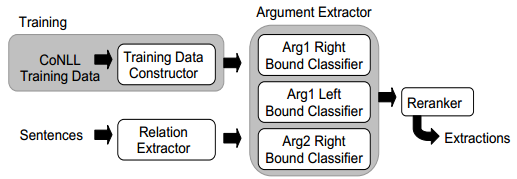
\includegraphics[scale=0.5]{../images/arglearner_architecture.png}
\caption{ArgLearner architecture training and extraction architecture}
\label{fig_arglearner_architecture}
\end{figure}

Furthermore, \textbf{Ollie} (Open Language Learning for Information Extraction) \citep{schmitz2012open} utilizes ReVerb \citep{fader2011identifying} to learn open pattern templates to guide triples extraction from sentence. Additionally, Ollie does a context analysis to extend the tuples with contextual information in order to improve precision \citep{schmitz2012open}. Its training and extraction architecture is describe in Figure \ref{fig_ollie_architecture}.

\begin{figure}
\centering
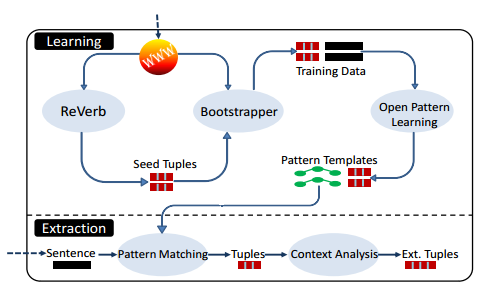
\includegraphics[scale=0.5]{../images/ollie_architecture.png}
\caption{Ollie labeling and extraction architecture}
\label{fig_ollie_architecture}
\end{figure}

One of the most research proposes new open IE system that replaces the usage of large open patterns in Ollie \citep{schmitz2012open} with a set of fewer patterns for canonically structured sentences and a classifier that learns to extract self-contained clauses from a sentence \citep{angeli2015leveraging}. This system is implemented in \textbf{Stanford OpenIE} which is also integrated in the populer open source suites, Stanford Core NLP.

%-----------------------------------------------------------------------------%
\section{\textit{Open Domain Information Extraction}}
%-----------------------------------------------------------------------------%

\lipsum[2-3]

%-----------------------------------------------------------------------------%
\section{\textit{Natural Language Processing}}
%-----------------------------------------------------------------------------%

\lipsum[3]

\subsection{CONLL-U}

\lipsum[4]

\subsection{\textit{Part of Speech Tagging}}

\lipsum[4]

\subsection{\textit{Named-Entity Recognition}}

\lipsum[5]

\subsection{\textit{Dependency Parsing}}

\lipsum[6]

%-----------------------------------------------------------------------------%
\section{\textit{Supervised Learning}}
%-----------------------------------------------------------------------------%

\lipsum[3]

\subsection{\textit{Logistic Regression}}

\lipsum[4]

\subsection{\textit{Support Vector Machine}}

\lipsum[5]

\subsection{\textit{Multi-Layer Perceptron}}

\lipsum[6]

\subsection{\textit{Random Forest}}

\lipsum[7]

\subsection{\textit{Cross Validation}}

\lipsum[8]
